\documentclass[border=10pt]{standalone}

\usepackage{tikz}
\usepackage{tikzsymbols}
\usetikzlibrary{calc,patterns,shapes.geometric}

\def\centerarc[#1](#2)(#3:#4:#5){\draw[#1] ($(#2)+({#5*cos(#3)},{#5*sin(#3)})$) arc (#3:#4:#5);}

\begin{document}
	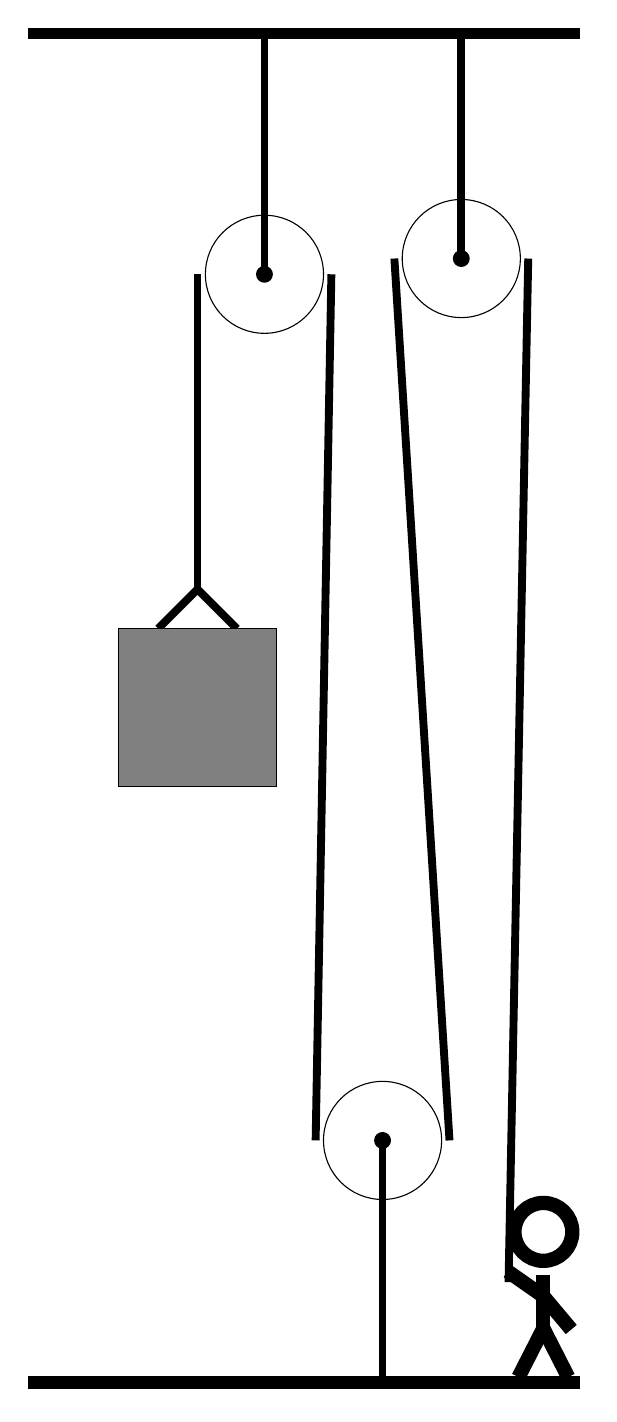
\begin{tikzpicture}
		%%%%% START %%%%%
		\draw[fill=black] (-2, 14) rectangle (5, 14.125);
		
		\draw (1, 11) circle (0.75);
		\draw[fill=black] (1, 11) circle (0.1);
		\draw[line width=1mm]  (1, 14) -- (1, 11);
		
		\draw[fill=white](2.5, 0) circle (0.75);
		\draw[fill=black] (2.5, 0) circle (0.1);
		\draw[line width=1mm]  (2.5, -3) -- (2.5, 0);
		
		\draw[fill=white](3.5, 11.2) circle (0.75);
		\draw[fill=black] (3.5, 11.2) circle (0.1);
		\draw[line width=1mm] (3.5, 14) -- (3.5, 11.2);
		
		\draw[line width=1mm] (-0.35, 6.5) -- (0.15, 7.0) -- (0.65, 6.5);
		\draw[fill=black!50] (-0.85, 6.5) rectangle (1.15, 4.5);
		
		\draw[line width=1mm] (0.15, 11) -- (0.15, 7.0);
		\centerarc[line width=1mm](1, 11)(0:180:0.85);
		\draw[line width=1mm](1.85, 11) -- (1.65, 0);
		\centerarc[line width=1mm](2.5, 0)(180:360:0.85);
		\draw[line width=1mm](3.35, 0) -- (2.65, 11.2);
		\centerarc[line width=1mm](3.5, 11.2)(0:180:0.85);
		\draw[line width=1mm](4.35, 11.2) -- (4.1, -1.8);
		
		\node at (4.5, -1.9) {\Strichmaxerl[10][-35][-50]};
		
		\draw[fill=black] (-2, -3) rectangle (5, -3.15);
		%%%%% END %%%%%
	\end{tikzpicture}
\end{document}